\flushbottom

%% CONTINUE: Added hint/solution links.


%%============================================================================
%%============================================================================
\chapter{Waves}








\raggedbottom
\exercises{
%%=============================================================================
\pagebreak
\flushbottom
\section{Exercises}








\begin{Exercise}
  Consider the 1-D wave equation 
  \[ 
  u_{t t} -  u_{x x} = 0 
  \] 
  on the domain $0 < x < 4$ with initial displacement 
  \[ 
  u(x,0) = \begin{cases}
    1, &1 < x < 2 \\ 
    0, &\mathrm{otherwise},
  \end{cases}
  \] 
  initial velocity $u_t(x,0) = 0$, and subject to the following boundary 
  conditions
  \begin{enumerate} 
  \item
    \[ 
    u(0,t) = u(4,t) = 0 
    \]
  \item
    \[ 
    u_x(0,t) = u_x(4,t) = 0
    \]
  \end{enumerate}
  In each case plot $u(x,t)$ for $t = \frac{1}{2}, 1, \frac{3}{2}, 2$ 
  and combine onto a general plot in the $x,t$ plane (up to a sufficiently 
  large time) so the behavior of $u$ is clear for arbitrary $x, t$. 
\end{Exercise}










%% Sketch the solution to the wave equation:
\begin{Exercise}
  Sketch the solution to the wave equation:
  \[
  u(x,t) = \frac{1}{2} \left( u(x+ct,0) + u(x-ct,0)\right) + 
  \frac{1}{2c} \int_{x-ct}^{x+ct} u_t(\tau,0) \,d\tau,
  \]
  for various values of $t$ corresponding to the initial conditions:
  \begin{enumerate}
  \item 
    $ \displaystyle u(x,0) = 0,\qquad u_t(x,0) = \sin \omega x \quad$ where
    $\omega$ is a constant, 
  \item 
    $ \displaystyle 
    u(x,0) = 0, \qquad 
    u_t(x,0) = 
    \begin{cases}
      1       &\mathrm{for}\ 0 < x < 1 \\
      -1      &\mathrm{for}\ -1 < x < 0 \\
      0       &\mathrm{for}\ |x|  > 1 .
    \end{cases}
    $
  \end{enumerate}
\end{Exercise}



%% Method of images: semi-infinite, finite interval.
\begin{Exercise}
  \begin{enumerate}
  \item 
    Consider the solution of the wave equation for $u(x,t)$:
    \[
    u_{tt} = c^2 u_{xx}
    \]
    on the infinite interval $-\infty < x < \infty$ with initial
    displacement of the form
    \[
    u(x,0) = 
    \begin{cases}
      h(x)    &\mathrm{for}\ x > 0, \\
      -h(-x)  &\mathrm{for}\ x < 0,
    \end{cases}
    \]
    and with initial velocity
    \[
    u_t(x,0) = 0.
    \]
    Show that the solution of the wave equation satisfying these initial
    conditions also solves the following semi-infinite problem: Find $u(x,t)$
    satisfying the wave equation $u_{tt} = c^2 u_{xx}$
    in $0 < x < \infty$, $ t > 0$, with initial conditions $u(x,0) = h(x)$,
    $u_t(x,0) = 0$, and with the fixed end condition $u(0,t) = 0$. Here $h(x)$ is 
    any given function with $h(0) = 0$. 
  \item 
    Use a similar idea to explain how you could use the general 
    solution of the wave equation to solve the finite interval problem
    $(0 < x < l)$ 
    in which $u(0,t) = u(l,t) = 0$ for all $t$, with $u(x,0) = h(x)$ and
    $u_t(x,0) = 0$. Take $h(0) = h(l) = 0$.
  \end{enumerate}
\end{Exercise}




%% Forward, backward.
\begin{Exercise}
  The deflection $u(x,T) = \phi(x)$ and 
  velocity $u_t(x,T) = \psi(x)$ for an infinite string (governed by
  $u_{tt} = c^2u_{xx}$) are measured at time $T$, and we are asked to determine
  what the initial displacement and velocity profiles $u(x,0)$ and
  $u_t(x,0)$ must have been. An alert student suggests that this problem is
  equivalent to that of determining the solution of the wave equation
  at time $T$ when initial conditions $u(x,0) = \phi(x)$, $u_t(x,0) = 
  -\psi(x)$ are prescribed. Is she correct? If not, can you rescue her idea?
\end{Exercise}




%% Consider the ``whip-cracking'' problem.
\begin{Exercise}
  In obtaining the general solution of the
  wave equation the interval was chosen to be infinite in order to simplify
  the evaluation of the functions $\alpha(\xi)$ and $\beta(\xi)$ in the 
  general solution
  \[
  u(x,t) = \alpha(x+ct) + \beta(x-ct).  
  \]
  But this general solution is in fact valid for any interval be it infinite
  or finite. We need only choose appropriate functions
  $\alpha(\xi)$, $\beta(\xi)$ to satisfy the appropriate initial and
  boundary conditions. This is not 
  always convenient but there are other situations besides the solution
  for $u(x,t)$ in an infinite domain in which the general solution is of use.
  Consider the ``whip-cracking'' problem,
  \[
  u_{tt} = c^2 u_{xx},  
  \]
  (with $c$ a constant) in the domain $x>0, t> 0$ with initial conditions
  \[
  u(x,0) = u_t(x,0) = 0 \qquad x>0,
  \]
  and boundary conditions
  \[
  u(0,t) = \gamma(t)
  \]
  prescribed for all $t> 0$. Here $\gamma(0) = 0$. Find $\alpha$ and $\beta$
  so as to determine $u$ for $x > 0$, $ t > 0.$ \\ \\
  \textit{Hint: } 
  (From physical considerations conclude that you can take $\alpha(\xi) = 0$.
  Your solution will corroborate this.)
  Use the initial conditions to determine 
  $\alpha(\xi)$ and $\beta(\xi)$ for $\xi > 0$.  Then use the initial
  condition to determine $\beta(\xi)$ for $\xi < 0$.
\end{Exercise}







%% Method of characteristics.
\begin{Exercise}
  Let $u(x,t)$ satisfy the equation 
  \[
  u_{tt} = c^2 u_{xx};    
  \]
  (with $c$ a constant) in some region of the $(x,t)$ plane.
  \begin{enumerate}
    %%
    %%
  \item 
    Show that the 
    quantity $(u_t - c u_x)$ is constant along each straight line defined
    by $x-ct = \mathrm{constant}$, and that $(u_t + cu_x)$ is constant along
    each straight line of the form $x+ct = \mathrm{constant}$. These
    straight lines 
    are called \textit{characteristics}; we will refer to typical members
    of the two families as $C_+$ and $C_-$ characteristics, respectively. Thus
    the line $x-ct = \mathrm{constant}$ is a $C_+$ characteristic.
    %%
    %%
  \item 
    Let $u(x,0)$ and $u_t(x,0)$ be prescribed for all values of
    $x$ in $-\infty < x < \infty$, and let  $(x_0,t_0)$ be some point
    in the $(x,t)$ plane, with $t_0 >0$. Draw the $C_+$ and $C_-$
    characteristics 
    through $(x_0,t_0)$ and let them intersect the $x$-axis at the points
    $A$,$B$. Use the properties of these curves derived in part (a) to
    determine 
    $u_t(x_0,t_0)$ in terms of initial data at points $A$ and $B$. Using 
    a similar technique to obtain $u_t(x_0,\tau)$ with $ 0 < \tau <t$, 
    determine 
    $u(x_0,t_0)$ by integration with respect to $\tau$, and compare this
    with the solution derived in class:
    \[
    u(x,t) = \frac{1}{2} \left( u(x+ct,0) + u(x-ct,0)\right) + 
    \frac{1}{2c} \int_{x-ct}^{x+ct} u_t(\tau,0) d\tau .
    \]
    Observe that this ``method of characteristics'' again shows that $u(x_0,t_0)$
    depends only on that part of the initial data between points $A$ and $B$.
  \end{enumerate}
\end{Exercise}






%% Temperature of the Earth's crust.
\begin{Exercise}
  The temperature $u(x,t)$ at a depth $x$ below the Earth's surface
  at time $t$ satisfies 
  \[
  u_t = \kappa u_{x x}.
  \]
  The surface $x = 0$ is heated by the sun according to the periodic rule:
  \[
  u(0,t) = T \cos( \omega t ).
  \]
  Seek a solution of the form
  \[
  u(x,t) = \Re \left( A \e^{\imath \omega t - \alpha x} \right).
  \]
  \begin{itemize}
    %%
  \item[a)]
    Find $u(x,t)$ satisfying $u \to 0$ as $x \to +\infty$, (i.e. deep into the
    Earth).  
    %%
  \item[b)]
    Find the temperature variation at a fixed depth, $h$, below the surface.
    %%
  \item[c)]
    Find the phase lag $\delta(x)$ such that when the maximum temperature
    occurs at $t_0$ on the surface, the maximum at depth $x$ occurs at 
    $t_0 + \delta(x)$.
    %%
  \item[d)]
    Show that the seasonal, (i.e. yearly), temperature changes and daily 
    temperature changes penetrate to depths in the ratio:
    \[
    \frac{ x_{\mathrm{year}} }{ x_{\mathrm{day}} } = \sqrt{365},
    \]
    where $x_{\mathrm{year}}$ and $x_{\mathrm{day}}$ are the depths of same
    temperature variation caused by the different periods of the source.
  \end{itemize}
\end{Exercise}










%% Infinite cylinder produces acoustic pressure field.
\begin{Exercise}
  An infinite cylinder of radius $a$ produces an external acoustic pressure
  field $u$ satisfying:
  \[
  u_{t t} = c^2 \delta u,
  \]
  by a pure harmonic oscillation of its surface at $r = a$.  That is, it moves 
  so that
  \[
  u(a, \theta, t) = f(\theta) \e^{\imath \omega t}
  \]
  where $f(\theta)$ is a known function.  Note that the waves must be outgoing
  at infinity, (radiation condition at infinity).  Find the solution, 
  $u(r, \theta, t)$.
  We seek a periodic solution of the form,
  \[
  u(r, \theta, t) = v(r, \theta) \e^{\imath \omega t}.
  \]
\end{Exercise}








%% Plane waves incident on a soft cylinder.
\begin{Exercise}
  Plane waves are incident on a ``soft'' cylinder of radius $a$ whose axis
  is parallel to the plane of the waves.  Find the field scattered by the 
  cylinder.  In particular, examine the leading term of the solution when
  $a$ is much smaller than the wavelength of the incident waves.
  If $v(x, y, t)$ is the scattered field it must satisfy:
  \begin{alignat*}{2}
    &\mathrm{Wave Equation:} &\quad &v_{t t} = c^2 \Delta v, \quad x^2 + y^2 > a^2;\\
    &\mathrm{Soft Cylinder:} &\quad &v(x, y, t) 
    = - \e^{\imath (k a \cos \theta - \omega t)},\ \mathrm{on}\ 
    r = a, \quad 0 \leq \theta < 2\pi; \\
    &\mathrm{Scattered:} &\quad &v\ \mathrm{is outgoing as}\ r \to \infty.
  \end{alignat*}
  Here $k = \omega / c$.  Use polar coordinates in the $(x, y)$ plane.
\end{Exercise}











%% Transmission line, telegrapher's system, traveling waves
\begin{Exercise}
  Consider the flow of electricity in a transmission line.  The current,
  $I(x, t)$, and the voltage, $V(x, t)$, obey the telegrapher's system of 
  equations:
  \begin{gather*}
    -I_x = C V_t + G V, \\
    -V_x = L I_t + R I,
  \end{gather*}
  where $C$ is the capacitance, $G$ is the conductance, $L$ is the inductance
  and $R$ is the resistance.

  \textbf{a)}  Show that both $I$ and $V$ satisfy a damped wave equation.

  \textbf{b)}  Find the relationship between the physical constants, $C$, $G$,
  $L$ and $R$ such that there exist damped traveling wave solutions of the
  form:
  \[
  V(x, t) = \e^{-\gamma t} (f(x - a t) + g(x + a t)).
  \]
  What is the wave speed?
\end{Exercise}






\raggedbottom
}
%%=============================================================================
\hints{
\pagebreak
\flushbottom
\section{Hints}






\begin{Hint}
  %% CONTINUE
\end{Hint}








%% Sketch the solution to the wave equation:
\begin{Hint}
  %% CONTINUE
\end{Hint}







%% Method of images: semi-infinite, finite interval.
\begin{Hint}
  %% CONTINUE
\end{Hint}




%% Forward, backward.
\begin{Hint}
  %% CONTINUE
\end{Hint}







%% Consider the ``whip-cracking'' problem.
\begin{Hint}
  From physical considerations conclude that you can take $\alpha(\xi) = 0$.
  Your solution will corroborate this.
  Use the initial conditions to determine 
  $\alpha(\xi)$ and $\beta(\xi)$ for $\xi > 0$.  Then use the initial
  condition to determine $\beta(\xi)$ for $\xi < 0$.
\end{Hint}







%% Method of characteristics.
\begin{Hint}
  %% CONTINUE
\end{Hint}




%% Temperature of the Earth's crust.
\begin{Hint} $\phantom{a}$ \\
  \begin{itemize}
    %%
  \item[a)]
    Substitute $u(x,t) = \Re(A \e^{\imath \omega t - \alpha x})$ into the partial 
    differential equation and solve for $\alpha$.  Assume that $\alpha$ has 
    positive real part so that the solution vanishes as $x \to +\infty$.
  \end{itemize}
\end{Hint}






%% Infinite cylinder produces acoustic pressure field.
\begin{Hint}
  Seek a periodic solution of the form,
  \[
  u(r, \theta, t) = v(r, \theta) \e^{\imath \omega t}.
  \]
  Solve the Helmholtz equation for $v$ with a Fourier series expansion,
  \[
  v(r, \theta) = \sum_{n = -\infty}^\infty v_n(r) \e^{\imath n \theta}.
  \]
  You will find that the $v_n$ satisfy Bessel's equation.  Choose the $v_n$
  so that $u$ satisfies the boundary condition at $r = a$ and the radiation 
  condition at infinity.  

  The Bessel functions have the asymptotic behavior,
  \begin{alignat*}{2}
    &J_n(\rho) \sim \sqrt{ \frac{2}{\pi\rho} } \cos(\rho - n \pi/2 - \pi/4), \quad
    &\mathrm{as}\ \rho \to \infty, \\
    &Y_n(\rho) \sim \sqrt{ \frac{2}{\pi\rho} } \sin(\rho - n \pi/2 - \pi/4), \quad
    &\mathrm{as}\ \rho \to \infty, \\
    &H_n^{(1)}(\rho) \sim \sqrt{ \frac{2}{\pi\rho} } \e^{i(\rho - n \pi/2 - \pi/4)}
    ,\quad &\mathrm{as}\ \rho \to \infty, \\
    &H_n^{(2)}(\rho) \sim \sqrt{ \frac{2}{\pi\rho} } \e^{-i(\rho- n \pi/2 - \pi/4)}
    ,\quad &\mathrm{as}\ \rho \to \infty.
  \end{alignat*}
\end{Hint}















%% Plane waves incident on a soft cylinder.
\begin{Hint}
  %% CONTINUE
\end{Hint}







%% Transmission line, telegrapher's system, traveling waves
\begin{Hint}
  %% CONTINUE
\end{Hint}








\raggedbottom
}
%%=============================================================================
\solutions{
\pagebreak
\flushbottom
\section{Solutions}







\begin{Solution}
  \begin{enumerate} 
  \item
    The initial position is 
    \[
    u(x,0) = H \left( \frac{1}{2} - \left| x - \frac{3}{2} \right| \right).
    \]
    We extend the domain of the problem to $(-\infty \ldots \infty)$ and add image sources 
    in the initial condition so that $u(x,0)$ is odd about $x = 0$ and 
    $x = 4$.  This enforces the boundary conditions at these two points.
    \begin{gather*}
      u_{t t} - u_{x x} = 0, \quad x \in (-\infty \ldots \infty), \quad t \in (0 \ldots \infty)
      \\
      u(x,0) = \sum_{n = - \infty}^\infty \left(
        H \left( \frac{1}{2} - \left| x - \frac{3}{2}  - 8 n \right| \right)
        - H \left( \frac{1}{2} - \left| x - \frac{13}{2}  - 8 n \right| \right)
      \right), \quad
      u_t(x,0) = 0
    \end{gather*}
    We use D'Alembert's solution to solve this problem.
    \begin{multline*}
      u(x,t) = \frac{1}{2} \sum_{n = - \infty}^\infty \left(
        H \left( \frac{1}{2} - \left| x - \frac{3}{2}  - 8 n - t \right| \right)
        + H \left( \frac{1}{2} - \left| x - \frac{3}{2}  - 8 n + t \right| \right)
      \right.
      \\
      \left.
        - H \left( \frac{1}{2} - \left| x - \frac{13}{2}  - 8 n - t \right| \right)
        - H \left( \frac{1}{2} - \left| x - \frac{13}{2}  - 8 n + t \right| \right)
      \right)
    \end{multline*}
    The solution at times: $t = 1/2, 1, 3/2, 2$ is plotted in 
    Figure~\ref{u0u40}.
    Note that the solution is periodic in time with period $8$.  
    Figure~\ref{phaseu0u40} shows the solution in the phase plane for 
    $0 < t < 8$.  Note the odd reflections at the boundaries.
    \begin{figure}[h!]
      \begin{center}
        \includegraphics[width=0.6\textwidth]{pde/waves/u0u40}
      \end{center}
      \caption{The solution at various times for the Dirichlet boundary 
        conditions.}
      \label{u0u40}
    \end{figure}

  \item
    The initial position is 
    \[
    u(x,0) = H \left( \frac{1}{2} - \left| x - \frac{3}{2} \right| \right).
    \]
    We extend the domain of the problem to $(-\infty \ldots \infty)$ and add image sources 
    in the initial condition so that $u(x,0)$ is even about $x = 0$ and 
    $x = 4$.  This enforces the boundary conditions at these two points.
    \begin{gather*}
      u_{t t} - u_{x x} = 0, \quad x \in (-\infty \ldots \infty), \quad t \in (0 \ldots \infty)
      \\
      u(x,0) = \sum_{n = - \infty}^\infty \left(
        H \left( \frac{1}{2} - \left| x - \frac{3}{2}  - 8 n \right| \right)
        + H \left( \frac{1}{2} - \left| x - \frac{13}{2}  - 8 n \right| \right)
      \right), \quad
      u_t(x,0) = 0
    \end{gather*}
    We use D'Alemberts solution to solve this problem.
    \begin{multline*}
      u(x,t) = \frac{1}{2} \sum_{n = - \infty}^\infty \left(
        H \left( \frac{1}{2} - \left| x - \frac{3}{2}  - 8 n - t \right| \right)
        + H \left( \frac{1}{2} - \left| x - \frac{3}{2}  - 8 n + t \right| \right)
      \right.
      \\
      \left.
        + H \left( \frac{1}{2} - \left| x - \frac{13}{2}  - 8 n - t \right| \right)
        + H \left( \frac{1}{2} - \left| x - \frac{13}{2}  - 8 n + t \right| \right)
      \right)
    \end{multline*}
    The solution at times $t = 1/2, 1, 3/2, 2$ is plotted in 
    Figure~\ref{ux0ux40}.
    Note that the solution is periodic in time with period $8$.  
    Figure~\ref{phaseu0u40} shows the solution in the phase plane for 
    $0 < t < 8$.  Note the even reflections at the boundaries.
    \begin{figure}[h!]
      \begin{center}
        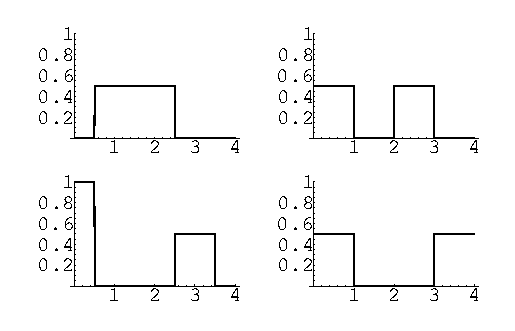
\includegraphics[width=0.6\textwidth]{pde/waves/ux0ux40}
      \end{center}
      \caption{The solution at various times for the Neumann boundary 
        conditions.}
      \label{ux0ux40}
    \end{figure}
  \end{enumerate}


  \begin{figure}[h!]
    \begin{center}
      \includegraphics[width=0.6\textwidth]{pde/waves/phaseu0u40}
    \end{center}
    \caption{The solution in the phase plane for the Dirichlet and
      Neumann boundary conditions.}
    \label{phaseu0u40}
  \end{figure}
\end{Solution}











%% Sketch the solution to the wave equation:
\begin{Solution}
  \begin{enumerate}
    %%
    %%
  \item
    \begin{gather*}
      u(x,t) = \frac{1}{2} \left( u(x+ct,0) + u(x-ct,0)\right) + 
      \frac{1}{2c} \int_{x-ct}^{x+ct} u_t(\tau,0) \,d\tau \\
      u(x,t) = \frac{1}{2c} \int_{x-ct}^{x+ct} \sin(\omega \tau) \,d\tau \\
      u(x,t) = \frac{ \sin(\omega x) \sin(\omega c t) }{ \omega c }
    \end{gather*}
    Figure~\ref{wave_ut_sin} shows the solution for $c = \omega = 1$.
    \begin{figure}[h!]
      \begin{center}
        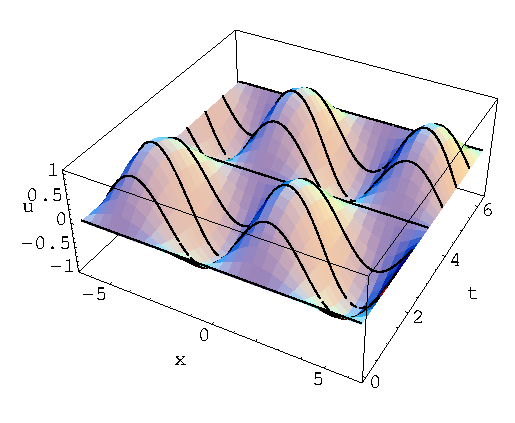
\includegraphics[width=0.5\textwidth]{pde/waves/wave_ut_sin}
      \end{center}
      \caption{Solution of the wave equation.}
      \label{wave_ut_sin}
    \end{figure}
    %%
    %%
  \item
    We can write the initial velocity in terms of the Heaviside function.
    \begin{gather*}
      u_t(x,0) = 
      \begin{cases}
        1       &\mathrm{for}\ 0 < x < 1 \\
        -1      &\mathrm{for}\ -1 < x < 0 \\
        0       &\mathrm{for}\ |x|  > 1 .
      \end{cases} \\
      u_t(x,0) = -H(x+1) + 2 H(x) - H(x-1)
    \end{gather*}
    We integrate the Heaviside function.
    \[
    \int_a^b H(x-c) \,d x = 
    \begin{cases}
      0 &\mathrm{for}\ b < c \\
      b-a &\mathrm{for}\ a > c \\
      b-c &\mathrm{otherwise}
    \end{cases}
    \]
    If $a < b$, we can express this as
    \[
    \int_a^b H(x-c) \,d x = \min( b-a, \max( b-c, 0 ) ).
    \]
    Now we find an expression for the solution.
    \begin{gather*}
      u(x,t) = \frac{1}{2} \left( u(x+ct,0) + u(x-ct,0)\right) + 
      \frac{1}{2c} \int_{x-ct}^{x+ct} u_t(\tau,0) \,d\tau 
      \\
      u(x,t) = \frac{1}{2c} \int_{x-ct}^{x+ct} \left(
        -H(\tau+1) + 2 H(\tau) - H(\tau-1) \right) \,d\tau
    \end{gather*}
    \begin{multline*}
      u(x,t) = - \min( 2 c t, \max( x + c t + 1, 0 ) )
      + 2 \min( 2 c t, \max( x + c t, 0 ) )
      \\
      - \min( 2 c t, \max( x + c t - 1, 0 ) )
    \end{multline*}
    Figure~\ref{wave_ut_du} shows the solution for $c = 1$.
    \begin{figure}[h!]
      \begin{center}
        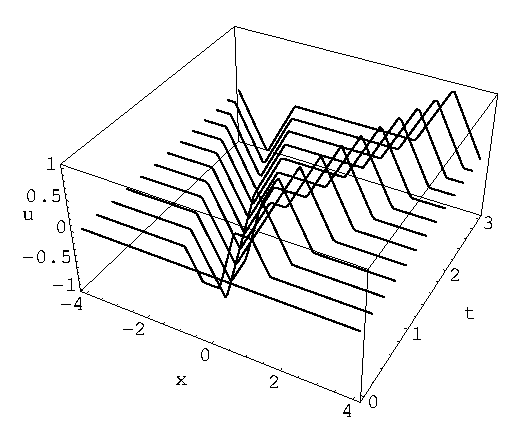
\includegraphics[width=0.5\textwidth]{pde/waves/wave_ut_du}
      \end{center}
      \caption{Solution of the wave equation.}
      \label{wave_ut_du}
    \end{figure}
  \end{enumerate}
\end{Solution}









%% Method of images: semi-infinite, finite interval.
\begin{Solution}
  \begin{enumerate}
    %%
    %%
  \item
    The solution on the interval $(-\infty \ldots \infty)$ is
    \[
    u(x,t) = \frac{1}{2} (h(x + c t) + h(x - c t)).
    \]
    Now we solve the problem on $(0 \ldots \infty)$.  We define the odd
    extension of $h(x)$.
    \[
    \hat{h}(x) = 
    \begin{cases}
      h(x)    &\mathrm{for}\ x > 0, \\
      -h(-x)  &\mathrm{for}\ x < 0,
    \end{cases}
    = \sign(x) h(|x|)
    \]
    Note that 
    \[
    \hat{h}'(0^-) = \frac{\dd}{\dd x}(-h(-x)) \big|_{x \to 0^+} = h'(0^+) 
    = \hat{h}'(0^+).
    \]
    Thus $\hat{h}(x)$ is piecewise $C^2$.  Clearly
    \[
    u(x,t) = \frac{1}{2} (\hat{h}(x + c t) + \hat{h}(x - c t))
    \]
    satisfies the differential equation on $(0 \ldots \infty)$. We
    verify that it satisfies the initial condition and boundary condition.
    \begin{gather*}
      u(x,0) = \frac{1}{2} (\hat{h}(x) + \hat{h}(x)) = h(x) \\
      u(0,t) = \frac{1}{2} (\hat{h}(c t) + \hat{h}(- c t))
      = \frac{1}{2} (h(c t) - h(c t))
      = 0
    \end{gather*}
    %%
    %%
  \item
    First we define the odd extension of $h(x)$ on the interval 
    $(-l \ldots l)$.
    \[
    \hat{h}(x) = \sign(x) h(|x|), \quad x \in (-l \ldots l)
    \]
    Then we form the odd periodic extension of $h(x)$ defined on
    $(-\infty \ldots \infty)$.
    \[
    \hat{h}(x) = \sign \left( x - 2 l \left\lfloor 
        \frac{x+l}{2l} \right\rfloor \right) 
    h\left( \left| x - 2 l \left\lfloor 
          \frac{x+l}{2l} \right\rfloor \right| \right),
    \quad x \in (-\infty \ldots \infty)
    \]
    We note that $\hat{h}(x)$ is piecewise $C^2$.  
    Also note that $\hat{h}(x)$ is odd about the points $x = n l$,
    $n \in \mathbb{Z}$.  That is, $\hat{h}(n l - x) = - \hat{h}(n l + x)$.
    Clearly
    \[
    u(x,t) = \frac{1}{2} (\hat{h}(x + c t) + \hat{h}(x - c t))
    \]
    satisfies the differential equation on $(0 \ldots l)$. We
    verify that it satisfies the initial condition and boundary conditions.
    \begin{gather*}
      u(x,0) = \frac{1}{2} (\hat{h}(x) + \hat{h}(x)) \\
      u(x,0) = \hat{h}(x) \\
      u(x,0) =  \sign \left( x - 2 l \left\lfloor 
          \frac{x+l}{2l} \right\rfloor \right) 
      h\left( \left| x - 2 l \left\lfloor 
            \frac{x+l}{2l} \right\rfloor\right|\right)\\
      u(x,0) = h(x) \\
      u(0,t) = \frac{1}{2} (\hat{h}(c t) + \hat{h}(- c t))
      = \frac{1}{2} (\hat{h}(c t) - \hat{h}(c t))
      = 0 \\
      u(l,t) = \frac{1}{2} (\hat{h}(l + c t) + \hat{h}(l - c t))
      = \frac{1}{2} (\hat{h}(l + c t) - \hat{h}(l + c t))
      = 0 
    \end{gather*}
  \end{enumerate}
\end{Solution}





%% Forward, backward.
\begin{Solution}
  \textbf{Change of Variables.}
  Let $u(x,t)$ be the solution of the problem with
  deflection $u(x,T) = \phi(x)$ and velocity $u_t(x,T) = \psi(x)$.
  Define
  \[
  v(x,\tau) = u(x,T-\tau).
  \]
  We note that $u(x,0) = v(x,T)$.  $v(\tau)$ satisfies the wave equation.
  \[
  v_{\tau\tau} = c^2 v_{x x}
  \]
  The initial conditions for $v$ are
  \[
  v(x,0) = u(x,T) = \phi(x), \quad v_\tau(x,0) = -u_t(x,T) = -\psi(x).
  \]
  Thus we see that the student was correct.

  \textbf{Direct Solution.}
  D'Alembert's solution is valid for all $x$ and $t$.  We formally 
  substitute $t-T$ for $t$ in this solution to solve the problem with
  deflection $u(x,T) = \phi(x)$ and velocity $u_t(x,T) = \psi(x)$.
  \[
  u(x,t) = \frac{1}{2} \left( \phi(x+c(t-T)) + \phi(x-c(t-T)) \right) + 
  \frac{1}{2c} \int_{x-c(t-T)}^{x+c(t-T)} \psi(\tau) \,d\tau
  \]
  This satisfies the wave equation, because the equation is 
  shift-invariant.  It also satisfies the initial conditions.
  \begin{gather*}
    u(x,T) = \frac{1}{2} \left( \phi(x) + \phi(x) \right) + 
    \frac{1}{2c} \int_{x}^{x} \psi(\tau) \,d\tau
    = \phi(x) \\
    u_t(x,t) = \frac{1}{2} \left( c \phi'(x+c(t-T)) - c \phi'(x-c(t-T)) \right) + 
    \frac{1}{2} \left( \psi(x+c(t-T)) + \psi(x-c(t-T)) \right) \\
    u_t(x,T) = \frac{1}{2} \left( c \phi'(x) - c \phi'(x) \right) + 
    \frac{1}{2} \left( \psi(x) + \psi(x) \right) 
    = \psi(x) 
  \end{gather*}
\end{Solution}








%% Consider the ``whip-cracking'' problem.
\begin{Solution}
  Since the solution is a wave moving to the right, we conclude that 
  we could take $\alpha(\xi) = 0$.  Our solution will corroborate this.

  The form of the solution is
  \[
  u(x,t) = \alpha(x+ct) + \beta(x-ct).  
  \]
  We substitute the solution into the initial conditions.
  \begin{gather*}
    u(x,0) = \alpha(\xi) + \beta(\xi) = 0, \quad \xi > 0 \\
    u_t(x,0) = c \alpha'(\xi) - c \beta'(\xi) = 0, \quad \xi > 0
  \end{gather*}
  We integrate the second equation to obtain the system
  \begin{gather*}
    \alpha(\xi) + \beta(\xi) = 0, \quad \xi > 0, \\
    \alpha(\xi) - \beta(\xi) = 2 k, \quad \xi > 0,
  \end{gather*}
  which has the solution
  \[
  \alpha(\xi) = k, \quad \beta(\xi) = -k, \quad \xi > 0.
  \]
  Now we substitute the solution into the initial condition.
  \begin{gather*}
    u(0,t) = \alpha(c t) + \beta(- c t) = \gamma(t), \quad t > 0 \\
    \alpha(\xi) + \beta(-\xi) = \gamma(\xi/c), \quad \xi > 0 \\
    \beta(\xi) = \gamma(-\xi/c) - k, \quad \xi < 0
  \end{gather*}
  This determines $u(x,t)$ for $x > 0$ as it depends on
  $\alpha(\xi)$ only for $\xi > 0$.  The constant $k$ is arbitrary.
  Changing $k$ does not change $u(x,t)$.  For simplicity, we take
  $k = 0$.  
  \begin{gather*}
    u(x,t) = \beta(x - c t) \\
    u(x,t) = \begin{cases}
      0 &\mathrm{for}\ x - c t < 0 \\
      \gamma(t - x/c) &\mathrm{for}\ x - c t > 0
    \end{cases} \\
    \boxed{
      u(x,t) = \gamma(t - x/c) H(c t - x)
      }
  \end{gather*}
\end{Solution}






%% Method of characteristics.
\begin{Solution}
  \begin{enumerate}
    %%
    %%
  \item 
    We write the value of $u$ along the line $x - c t = k$ as a function 
    of $t$: $u(k+c t, t)$.  We differentiate $u_t - c u_x$ with respect
    to $t$ to see how the quantity varies.
    \begin{align*}
      \frac{\dd}{\dd t} \left( u_t(k+c t, t) - c u_x(k+c t, t) \right)
      &= c u_{x t} + u_{t t} - c^2 u_{x x} - c u_{x t} \\
      &= u_{t t} - c^2 u_{x x} \\
      &= 0
    \end{align*}
    Thus $u_t - c u_x$ is constant along the line $x - c t = k$.  Now we
    examine $u_t + c u_x$ along the line $x + c t = k$.  
    \begin{align*}
      \frac{\dd}{\dd t} \left( u_t(k-c t, t) + c u_x(k-c t, t) \right)
      &= - c u_{x t} + u_{t t} - c^2 u_{x x} + c u_{x t} \\
      &= u_{t t} - c^2 u_{x x} \\
      &= 0
    \end{align*}
    $u_t + c u_x$ is constant along the line $x + c t = k$. 
    %%
    %%
  \item 
    From part (a) we know
    \begin{gather*}
      u_t(x_0,t_0) - c u_x(x_0,t_0) = u_t(x_0-c t_0,0) - c u_x(x_0-c t_0,0) \\
      u_t(x_0,t_0) + c u_x(x_0,t_0) = u_t(x_0+c t_0,0) + c u_x(x_0+c t_0,0).
    \end{gather*}
    We add these equations to find $u_t(x_0,t_0)$.
    \[
    u_t(x_0,t_0) = \frac{1}{2} \left( u_t(x_0-c t_0,0) - c u_x(x_0-c t_0,0)
      u_t(x_0+c t_0,0) + c u_x(x_0+c t_0,0) \right)
    \]
    Since $t_0$ was arbitrary, we have
    \[
    u_t(x_0,\tau) = \frac{1}{2} \left( u_t(x_0-c \tau,0) - c u_x(x_0-c \tau,0)
      u_t(x_0+c \tau,0) + c u_x(x_0+c \tau,0) \right)
    \]
    for $0 < \tau < t_0$.  We integrate with respect to $\tau$ to 
    determine $u(x_0,t_0)$.
    \begin{align*}
      u(x_0,t_0) &= u(x_0,0) + \int_0^{t_0} \frac{1}{2} 
      \left( u_t(x_0-c \tau,0) - c u_x(x_0-c \tau,0)
        u_t(x_0+c \tau,0) + c u_x(x_0+c \tau,0) \right)\,d\tau \\
      &= u(x_0,0) + \frac{1}{2} \int_0^{t_0}
      \left( - c u_x(x_0-c \tau,0) + c u_x(x_0+c \tau,0)
      \right)\,d\tau \\
      &\qquad + \frac{1}{2} \int_0^{t_0}
      \left( u_t(x_0-c \tau,0) + u_t(x_0+c \tau,0) \right)\,d\tau \\
      &= u(x_0,0) + \frac{1}{2} \left( u(x_0-c t_0,0) - u(x_0,0) 
        + u(x_0+c t_0,0) - u(x_0,0) \right) \\
      &\qquad + \frac{1}{2c} \int_{x_0}^{x_0-c t_0} - u_t(\tau,0) \,d \tau 
      + \frac{1}{2c} \int_{x_0}^{x_0+c t_0} u_t(\tau,0) \,d\tau \\
      &= \frac{1}{2} \left( u(x_0-c t_0,0) + u(x_0+c t_0,0) \right)
      + \frac{1}{2c} \int_{x_0-c t_0}^{x_0+c t_0} 
      u_t(\tau,0) \,d\tau
    \end{align*}
    We have D'Alembert's solution.
    \[
    \boxed{
      u(x,t) = \frac{1}{2} \left( u(x-c t,0) + u(x+c t,0) \right)
      + \frac{1}{2c} \int_{x-c t}^{x+c t} u_t(\tau,0) \,d\tau
      }
    \]
  \end{enumerate}
\end{Solution}






%% Temperature of the Earth's crust.
\begin{Solution} $\phantom{a}$ \\
  \begin{itemize}
    %%
  \item[a)]
    We substitute $u(x,t) = A \e^{\imath \omega t - \alpha x}$ into the partial 
    differential equation and take the real part as the solution.  We assume
    that $\alpha$ has positive real part so the solution vanishes as
    $x \to +\infty$.
    \begin{gather*}
      \imath \omega A \e^{\imath \omega t - \alpha x} 
      = \kappa \alpha^2 A \e^{\imath \omega t - \alpha x} \\
      \imath \omega = \kappa \alpha^2 \\
      \alpha = (1 + \imath) \sqrt{ \frac{\omega}{2 \kappa} }
    \end{gather*}
    A solution of the partial differential equation is,
    \[
    u(x,t) = \Re \left( A \exp\left( \imath \omega t - (1 + \imath) \sqrt{
          \frac{\omega}{2\kappa} } x \right) \right),
    \]
    \[
    u(x,t) = A \exp\left( - \sqrt{ \frac{\omega}{2\kappa} } x \right) 
    \cos\left( \omega t - \sqrt{ \frac{\omega}{2\kappa} } x \right).
    \]
    Applying the initial condition, $u(0,t) = T \cos(\omega t)$, we obtain,
    \[
    \boxed{
      u(x,t) = T \exp\left( - \sqrt{ \frac{\omega}{2\kappa} } x \right) 
      \cos\left( \omega t - \sqrt{ \frac{\omega}{2\kappa} } x \right).
      }
    \]
    %%
  \item[b)]
    At a fixed depth $x = h$, the temperature is
    \[
    u(h,t) = T \exp\left( - \sqrt{ \frac{\omega}{2\kappa} } h \right) 
    \cos\left( \omega t - \sqrt{ \frac{\omega}{2\kappa} } h \right).
    \]
    Thus the temperature variation is
    \[
    \boxed{
      - T \exp\left( - \sqrt{ \frac{\omega}{2\kappa} } h \right) 
      \leq u(h,t) \leq
      T \exp\left( - \sqrt{ \frac{\omega}{2\kappa} } h \right).
      }
    \]
    %%
  \item[c)]
    The solution is an exponentially decaying, traveling wave that propagates 
    into the Earth with speed 
    $\omega/\sqrt{\omega/(2\kappa)} = \sqrt{ 2 \kappa \omega }$.
    More generally, the wave
    \[
    \e^{-b t} \cos(\omega t - a x)
    \]
    travels in the positive direction with speed $\omega / a$.
    Figure~\ref{decay_travel} shows such a wave for a sequence of times.

    \begin{figure}[h!]
      \begin{center}
        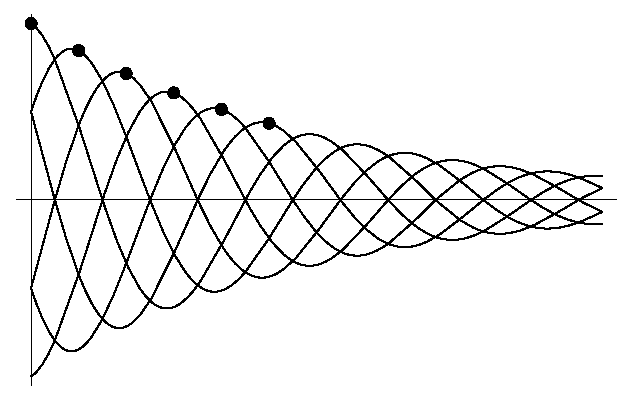
\includegraphics[width=0.5\textwidth]{pde/waves/decay_travel}
      \end{center}
      \caption{An exponentially decaying, traveling wave.}
      \label{decay_travel}
    \end{figure}

    The phase lag, $\delta(x)$ is the time that it takes for the wave to 
    reach a depth of $x$.  It satisfies,
    \[
    \omega \delta(x) - \sqrt{ \frac{\omega}{2 \kappa} } x = 0,
    \]
    \[
    \boxed{
      \delta(x) = \frac{x}{ \sqrt{ 2 \kappa \omega } }. 
      }
    \]
    %%
  \item[d)]
    Let $\omega_{\mathrm{year}}$ be the frequency for annual temperature variation,
    then $\omega_{\mathrm{day}} = 365 \omega_{\mathrm{year}}$.  If
    $x_{\mathrm{year}}$ is the depth that a particular yearly temperature
    variation reaches and $x_{\mathrm{day}}$ is the depth that this same 
    variation in daily temperature reaches, then
    \[
    \exp\left( - \sqrt{ \frac{ \omega_{\mathrm{year}} }{ 2 \kappa }}
      x_{\mathrm{year}} \right)
    = \exp\left( - \sqrt{ \frac{ \omega_{\mathrm{day}} }{ 2 \kappa }}
      x_{\mathrm{day}} \right),
    \]
    \[
    \sqrt{ \frac{ \omega_{\mathrm{year}} }{ 2 \kappa }}
    x_{\mathrm{year}} 
    = \sqrt{ \frac{ \omega_{\mathrm{day}} }{ 2 \kappa }}
    x_{\mathrm{day}},
    \]
    \[
    \boxed{
      \frac{ x_{\mathrm{year}} }{ x_{\mathrm{day}} } = \sqrt{365}.
      }
    \]
  \end{itemize}
\end{Solution}





%% Infinite cylinder produces acoustic pressure field.
\begin{Solution}
  We seek a periodic solution of the form,
  \[
  u(r, \theta, t) = v(r, \theta) \e^{\imath \omega t}.
  \]
  Substituting this into the wave equation will give us a Helmholtz equation for
  $v$.
  \begin{gather*}
    - \omega^2 v = c^2 \Delta v \\
    v_{r r} + \frac{1}{r} v_r + \frac{1}{r^2} v_{\theta\theta} 
    + \frac{\omega^2}{c^2} v = 0
  \end{gather*}
  We have the boundary condition $v(a, \theta) = f(\theta)$ and the radiation
  condition at infinity.  We expand $v$ in a Fourier series in $\theta$ in
  which the coefficients are functions of $r$.  You can check that 
  $\e^{\imath n \theta}$ are the eigenfunctions obtained with separation of 
  variables.
  \[
  v(r, \theta) = \sum_{n = -\infty}^\infty v_n(r) \e^{\imath n \theta}
  \]
  We substitute this expression into the Helmholtz equation to obtain ordinary
  differential equations for the coefficients $v_n$.
  \begin{gather*}
    \sum_{n = -\infty}^\infty \left( v_n'' + \frac{1}{r} v_n' + \left( \frac{\omega^2}{c^2}
        - \frac{n^2}{r^2} \right) v_n \right) \e^{\imath n \theta} = 0 \\
    \intertext{The differential equations for the $v_n$ are}
    v_n'' + \frac{1}{r} v_n' + \left( \frac{\omega^2}{c^2} - \frac{n^2}{r^2}
    \right) v_n = 0. \\
    \intertext{which has as linearly independent solutions the Bessel and 
      Neumann functions,}
    J_n \left( \frac{\omega r}{c} \right), \quad 
    Y_n \left( \frac{\omega r}{c} \right), \\
    \intertext{or the Hankel functions,}
    H_n^{(1)} \left( \frac{\omega r}{c} \right), \quad 
    H_n^{(2)} \left( \frac{\omega r}{c} \right). 
  \end{gather*}
  The functions have the asymptotic behavior,
  \begin{alignat*}{2}
    &J_n(\rho) \sim \sqrt{ \frac{2}{\pi\rho} } \cos(\rho - n \pi/2 - \pi/4), \quad
    &\mathrm{as}\ \rho \to \infty, \\
    &Y_n(\rho) \sim \sqrt{ \frac{2}{\pi\rho} } \sin(\rho - n \pi/2 - \pi/4), \quad
    &\mathrm{as}\ \rho \to \infty, \\
    &H_n^{(1)}(\rho) \sim \sqrt{ \frac{2}{\pi\rho} } \e^{i(\rho - n \pi/2 - \pi/4)}
    ,\quad &\mathrm{as}\ \rho \to \infty, \\
    &H_n^{(2)}(\rho) \sim \sqrt{ \frac{2}{\pi\rho} } \e^{-i(\rho- n \pi/2 - \pi/4)}
    ,\quad &\mathrm{as}\ \rho \to \infty.
  \end{alignat*}
  $u(r,\theta,t)$ will be an outgoing wave at infinity if it is the sum of 
  terms of the form $\e^{i(\omega t - \mathrm{const} r)}$.  Thus the $v_n$
  must have the form
  \[
  v_n(r) = b_n H_n^{(2)} \left( \frac{\omega r}{c} \right)
  \]
  for some constants, $b_n$.  The solution for $v(r,\theta)$ is
  \[
  v(r, \theta) = \sum_{n = -\infty}^\infty b_n H_n^{(2)} \left( \frac{\omega r}{c} \right) 
  \e^{\imath n \theta}.
  \]
  We determine the constants $b_n$ from the boundary condition at $r = a$.
  \begin{gather*}
    v(a, \theta) = \sum_{n = -\infty}^\infty b_n H_n^{(2)} \left( \frac{\omega a}{c} \right) 
    \e^{\imath n \theta} = f(\theta) \\
    \boxed{
      b_n = \frac{1}{2 \pi H_n^{(2)} (\omega a/c)} \int_0^{2\pi} f(\theta)
      \e^{-\imath n \theta} \,d\theta
      } \\
    \boxed{
      u(r, \theta, t) = \e^{\imath \omega t}
      \sum_{n = -\infty}^\infty b_n H_n^{(2)} \left( \frac{\omega r}{c} \right) \e^{\imath n \theta}
      }
  \end{gather*}
\end{Solution}















%% Plane waves incident on a soft cylinder.
\begin{Solution}
  We substitute the form $v(x, y, t) = u(r, \theta) \e^{-\imath \omega t}$ into
  the wave equation to obtain a Helmholtz equation.
  \begin{gather*}
    c^2 \Delta u + \omega^2 u = 0 \\
    u_{r r} + \frac{1}{r} u_r + \frac{1}{r^2} u_{\theta\theta} + k^2 u = 0
  \end{gather*}
  We solve the Helmholtz equation with separation of variables.  We expand
  $u$ in a Fourier series.
  \[
  u(r, \theta) = \sum_{n = -\infty}^\infty u_n(r) \e^{\imath n \theta}
  \]
  We substitute the sum into the Helmholtz equation to determine ordinary 
  differential equations for the coefficients.
  \[
  u_n'' + \frac{1}{r} u_n' + \left( k^2 - \frac{n^2}{r^2} \right) u_n = 0
  \]
  This is Bessel's equation, which has as solutions the Bessel and Neumann
  functions, $\{ J_n(k r), Y_n(k r) \}$ or the Hankel functions,
  $\{ H_n^{(1)}(k r), H_n^{(2)}(k r) \}$.

  Recall that the solutions of the Bessel equation have the asymptotic 
  behavior,
  \begin{alignat*}{2}
    &J_n(\rho) \sim \sqrt{ \frac{2}{\pi\rho} } \cos(\rho - n \pi/2 - \pi/4), \quad
    &\mathrm{as}\ \rho \to \infty, \\
    &Y_n(\rho) \sim \sqrt{ \frac{2}{\pi\rho} } \sin(\rho - n \pi/2 - \pi/4), \quad
    &\mathrm{as}\ \rho \to \infty, \\
    &H_n^{(1)}(\rho) \sim \sqrt{ \frac{2}{\pi\rho} } \e^{i(\rho - n \pi/2 - \pi/4)}
    ,\quad &\mathrm{as}\ \rho \to \infty, \\
    &H_n^{(2)}(\rho) \sim \sqrt{ \frac{2}{\pi\rho} } \e^{-i(\rho- n \pi/2 - \pi/4)}
    ,\quad &\mathrm{as}\ \rho \to \infty.
  \end{alignat*}
  From this we see that only the Hankel function of the first kink will give us
  outgoing waves as $\rho \to \infty$.  Our solution for $u$ becomes,
  \[
  u(r, \theta) = \sum_{n = -\infty}^\infty b_n H_n^{(1)}(k r) \e^{\imath n \theta}.
  \]
  We determine the coefficients in the expansion from the boundary condition
  at $r = a$.
  \begin{gather*}
    u(a, \theta) = \sum_{n = -\infty}^\infty b_n H_n^{(1)}(k a) \e^{\imath n \theta} 
    = - \e^{\imath k a \cos \theta} \\
    b_n = - \frac{1}{2 \pi H_n^{(1)}(k a)} \int_0^{2 \pi} \e^{\imath k a \cos \theta}
    \e^{-\imath n \theta} \,d \theta
  \end{gather*}
  We evaluate the integral with the identities,
  \begin{gather*}
    J_n(x) = \frac{1}{2 \pi i^n} \int_0^{2 \pi} \e^{\imath x \cos \theta} 
    \e^{\imath n \theta} \,d \theta, \\
    J_{-n}(x) = (-1)^n J_n(x).
  \end{gather*}
  Thus we obtain,
  \[
  \boxed{
    u(r, \theta) = - \sum_{n = -\infty}^\infty \frac{ (-\imath)^n J_n(k a)}{H_n^{(1)}(k a)}
    H_n^{(1)}(k r) \e^{\imath n \theta}.
    }
  \]
  When $a \ll 1/k$, i.e. $k a \ll 1$, the Bessel function has the behavior,
  \[
  J_n(k a) \sim \frac{(k a/2)^n}{n!}.
  \]
  In this case, the $n \neq 0$ terms in the sum are much smaller than the
  $n = 0$ term.  The approximate solution is,
  \begin{gather*}
    u(r, \theta) \sim - \frac{ H_0^{(1)}(k r) }{ H_0^{(1)}(k a) }, \\
    \boxed{
      v(r, \theta, t) \sim - \frac{ H_0^{(1)}(k r) }{ H_0^{(1)}(k a) } 
      \e^{-\imath \omega t}.
      }
  \end{gather*}
\end{Solution}














%% Transmission line, telegrapher's system, traveling waves
\begin{Solution}
  $\phantom{a}$

  \textbf{a)}
  \[
  \Bigg\{
  \begin{matrix}
    -I_x = C V_t + G V, \\
    -V_x = L I_t + R I
  \end{matrix}
  \]
  First we derive a single partial differential equation for $I$.
  We differentiate the two partial differential equations with respect to $x$
  and $t$, respectively and then eliminate the $V_{x t}$ terms. 
  \begin{gather*}
    \Bigg\{
    \begin{matrix}
      -I_{x x} = C V_{t x} + G V_x, \\
      -V_{x t} = L I_{t t} + R I_t
    \end{matrix} \\
    -I_{x x} + L C I_{t t} + R C I_t = G V_x \\
    \intertext{We use the initial set of equations to write $V_x$ in terms of $I$.}
    -I_{x x} + L C I_{t t} + R C I_t + G ( L I_t + R I ) = 0 \\
    \boxed{
      I_{t t} + \frac{R C + G L}{L C} I_t + \frac{G R}{L C} I - \frac{1}{L C} I_{x x}
      = 0
      }
  \end{gather*}

  Now we derive a single partial differential equation for $V$.
  We differentiate the two partial differential equations with respect to $t$
  and $x$, respectively and then eliminate the $I_{x t}$ terms. 
  \begin{gather*}
    \Bigg\{
    \begin{matrix}
      -I_{x t} = C V_{t t} + G V_t, \\
      -V_{x x} = L I_{t x} + R I_x
    \end{matrix} \\
    -V_{x x} = R I_x - L C V_{t t} - L G V_t \\
    \intertext{We use the initial set of equations to write $I_x$ in terms of $V$.}
    L C V_{t t} + L G V_t - V_{x x} + R (C V_t + G V) = 0 \\
    \boxed{
      V_{t t} + \frac{R C + L G}{L C} V_t + \frac{R G}{L C} V  
      - \frac{1}{L C} V_{x x} = 0.
      }
  \end{gather*}
  Thus we see that $I$ and $V$ both satisfy the same damped wave equation.

  \textbf{b)}
  We substitute $V(x, t) = \e^{-\gamma t} (f(x - a t) + g(x + a t))$ into the
  damped wave equation for $V$.
  \begin{multline*}
    \left( \gamma^2 - \frac{R C + L G}{L C} \gamma + \frac{R G}{L C} \right)
    \e^{- \gamma t} (f + g)
    + \left( - 2 \gamma + \frac{R C + L G}{L C} \right) a 
    \e^{- \gamma t} (-f' + g') \\
    + a^2 \e^{-\gamma t} (f'' + g'')
    - \frac{1}{L C} \e^{-\gamma t} (f'' + g'') = 0
  \end{multline*}
  Since $f$ and $g$ are arbitrary functions, the coefficients of 
  $\e^{-\gamma t}(f + g)$, $\e^{-\gamma t}(-f' + g')$ and
  $\e^{-\gamma t}(f'' + g'')$ must vanish.  This gives us three constraints.
  \[
  a^2 - \frac{1}{L C} = 0, \quad
  - 2 \gamma + \frac{R C + L G}{L C} = 0, \quad
  \gamma^2 - \frac{R C + L G}{L C} \gamma + \frac{R G}{L C} = 0
  \]
  The first equation determines the wave speed to be $a = 1/ \sqrt{L C}$.
  We substitute the value of $\gamma$ from the second equation into the third 
  equation.
  \[
  \gamma = \frac{R C + L G}{2 L C},\quad
  -\gamma^2 + \frac{R G}{L C} = 0
  \]
  In order for damped waves to propagate, the physical constants must satisfy,
  \begin{gather*}
    \frac{R G}{L C} - \left( \frac{R C + L G}{2 L C} \right)^2 = 0, \\
    4 R G L C - (R C + L G)^2 = 0, \\
    (R C - L G)^2 = 0, \\
    \boxed{
      R C = L G.
      }
  \end{gather*}
\end{Solution}










\raggedbottom
}
